\chapter{System Specification, Design, and Implementation}\label{ch:specs_design_implem}

This chapter presents the proposed solution, including four main sections.
Section~\ref{sec:specs} discusses the requirements and specifications, Section~\ref{sec:prop_vision} presents the proposed vision module.
Section~\ref{sec:design} explains the solution design.
Finally, Section~\ref{sec:impl} presents the implementation of the system.

\section{System Specification}\label{sec:specs}
The goal of this dissertation was to extract vision-based information relevant to a 5G network.
This information should be available in near real-time to relevant entities of the network architecture upon subscription.
This solution envisions obstacle-aware networks and should enable a RAN to autonomously control the BS' placement and configuration based on the environment perception provided by the vision-based information.

\subsection{System Requirements}\label{subsec:system-requirements}

To demonstrate these concepts, we conceptualized a simple model.
The scenario is set in an indoor office environment, where it is determined if common objects will impact the LOS between a gNB and a UE\@.

To achieve this, specific system requirements were established to ensure the efficient detection, tracking, and dissemination of obstacles information within the 5G network.

The detailed requirements of the Computer Vision Module and its interface with the network are as follows:

\begin{enumerate}
    \item \textbf{Functional Requirements}
    \begin{enumerate}
        \item Detect and track objects in near real-time using computer vision algorithms.
        \item Identify specific obstacles and predict potential blockages.
        \item Send well-defined messages to a novel O-RAN xApp for further processing and decision-making.
        \item Ensure interoperability with the 5G network components via standardized messaging protocols. % should i use standarized, since there is no standard for it, i created a structure?
    \end{enumerate}
    \item \textbf{Non-Functional Requirements}
    \begin{enumerate}
        \item Maximize processing speed resorting to parallel processing on the GPU whenever possible\@.
        \item Minimize messaging latency ensuring rapid response by the xApp for optimal connection maintenance.
        \item High accuracy in object detection and tracking to minimize false positives and negatives.
        \item The solution should be scalable to handle multiple video streams, Base Stations, and UEs, allowing for broader deployment in various network environments.
        \item The system must use standardized messaging formats to ensure interoperability with different network components and vendors.
        \item The vision module and communications system should be robust, with mechanisms for error detection and recovery to maintain continuous operation.
        The model and its parameters are fundamental to assuring reliability. % how can i prove it?
    \end{enumerate}
\end{enumerate}

These requirements translate into Table ~\ref{tab:spec}, containing system specifications:

\begin{table}[H]
\caption{System Specifications.}
\label{tab:spec}
\centering
\resizebox{\textwidth}{!}{%
\begin{tabular}{|l|p{12cm}|}
\hline
\textbf{Specification} & \textbf{Description} \\ \hline
\textbf{Detection and tracking} & Use YOLOv5 Ultralytics~\cite{Ultralytics_repo} and BoT-SORT~\cite{botsort} for high accuracy and optimized speed. \\ \hline
\textbf{Messaging} & Encode messages using ASN.1 standards. \newline Transmit messages via SCTP protocol. \newline Include relevant information such as object ID, type, position ( cartesian coordinates), and confidence score. \\ \hline
\end{tabular}}
\end{table}

These specifications ensure that the Vision Module meets the requirements necessary for integration and operation within a 5G network environment.


Following these requirements and specifications, the system architecture was designed to facilitate efficient data processing.

\begin{figure}[H]
    \centering
    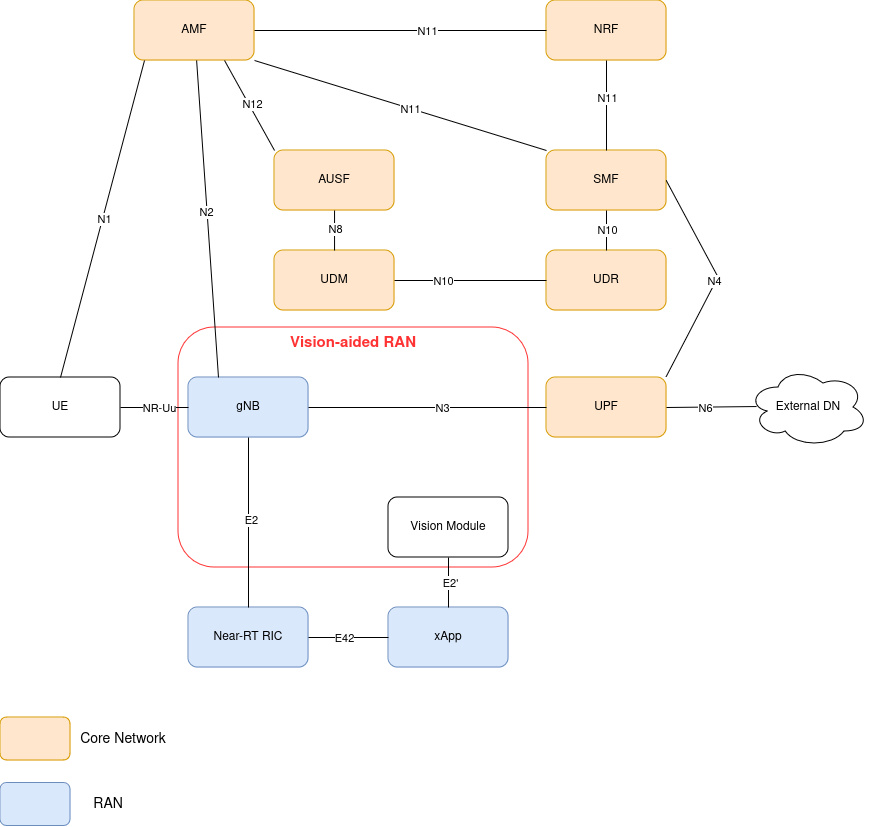
\includegraphics[width=0.7\linewidth]{figures/Syst_Arch.drawio}
    \caption[System Architecture of the proposed solution]{System Architecture of the proposed solution}
    \label{fig:my_arch}
\end{figure}

% draw: SMF[x], SPGWU[x], AMF[x], AUSF, UDM, UDR, mysql, NRF ext DN[x]
% requires improvements
In the proposed architecture, shown in Figure~\ref{fig:my_arch}, a UE requires 5G connectivity.
The 5G connection workflow begins with the UE initiating a connection request to the gNB, which then forwards the request to the AMF\@.
The gNB serves as the intermediary between the UE and the 5G core network, managing the radio resources, handling data transmission, and ensuring seamless connectivity as the UE moves.
The AMF authenticates the UE using credentials stored in the UDM. Upon successful authentication, the UE is granted access to the network.
The AMF and UPF then establish a data session for the UE, configuring the necessary resources for data transmission.
User data is transmitted between the UE and the UPF via the gNB\@.
The UPF routes the data to and from external networks, ensuring efficient data flow.

%------------ move to another place
%The 5G Core Network is responsible for managing the overall network functions, including authentication, mobility management, and routing of data.
%In our solution, both the RAN and the core are deployed within the same processing unit to maintain efficiency, mobility and simplicity.
%The AMF is a critical component of the 5G core that handles user authentication and mobility management.
%When a UE attempts to connect to the network, the AMF verifies the user's credentials and manages their session as they move across different cells in the network.

%The User Plane Function (UPF) manages the user data traffic, ensuring that data packets are efficiently routed between the UE and external data networks.
%It plays a pivotal role in delivering low-latency, high-bandwidth services to the end-users.
%Another essential core network function is the Unified Data Management (UDM), responsible for handling subscriber data and profiles.
%It ensures that user data is consistent and accessible across the network, supporting seamless user experiences.
%The User Plane Function (UPF) manages the user data traffic, ensuring that data packets are efficiently routed between the UE and external data networks.
%It plays a pivotal role in delivering low-latency, high-bandwidth services to the end-users.
%Another essential core network function is the Unified Data Management (UDM), responsible for handling subscriber data and profiles.
%It ensures that user data is consistent and accessible across the network, supporting seamless user experiences.

%To ensure the mobility and efficiency of our solution, the RAN and the core network components are deployed within the same processing unit.
%This integration offers several advantages.
%By colocating the RAN and core network functions, data processing and transmission delays are minimized, resulting in a more responsive network.
%The mobile RAN can seamlessly maintain connectivity with the UE, even when the gNB is moving, without relying on distant core network infrastructure.
%Having the RAN and core in a single unit simplifies the deployment process, making it easier to set up and manage the network in various locations, whether stationary or on the move.
%-------------------

In our solution, the RAN can be repositioned according to environment conditions that possibly affect the RF\@.
Those are reported by the Vision Module (Vision Module).
This enables the RAN to control manage its placement, based on those conditions together with radio metrics, such as SNR\@.
In order to establish the integration of Computer Vision into the 5G architecture, we took advantage of the Near-RT RIC, specified by O-RAN, to deploy a xApp responsible for the handling both radio metrics and the VM messages.
The communication between the VM and the xApp, is done through an interface inspired by the O-RAN E2 interface and E2 Application Protocol (E2AP).
This interface facilitates reliable data exchange using a SCTP socket connection (cf.Figure~\ref{fig:stack}) along with an Abstract Syntax Notation One (ASN.1) definition to structure the messages.
The use of ASN.1 ensures that the message formats are standardized, promoting interoperability and efficiency in data transmission.
This design allows the VM to communicate with the xApp, enabling the integration of data extracted from video for the mobile RAN management.

\begin{figure}[H]
    \centering
    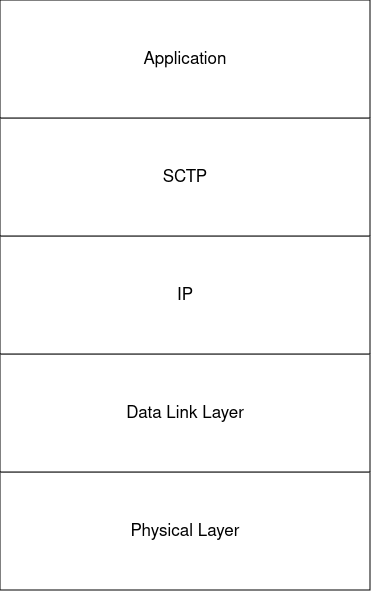
\includegraphics[width=0.35\linewidth]{figures/VisionModule_ProtocolStack.drawio(2)}
    \caption[Proposed Vision Module Protocol Stack]{Proposed vision module protocol stack.}
    \label{fig:stack}
\end{figure}


\section{Proposed Vision Module}\label{sec:prop_vision}
Our proposed vision module uses Computer Vision techniques to extract information about obstacles within the video camera's field of view.
This system processes video frames to detect and track obstacles, subsequently sending messages to services connected with relevant information.
The module sends five types of messages: blockage, future blockage, past blockage, the location of the UE and frame processed.
Table~\ref{tab:message_type} summarizes the description of each message type.
Each message will be explained further in the following sections.

\begin{table}[H]
    \caption{Summary of each message type}
    \label{tab:message_type}
    \centering
    \resizebox{\textwidth}{!}{%
        \begin{tabular}{|l|p{12cm}|}
            \hline
            \textbf{Type of message} & \textbf{Description} \\ \hline
            Blockage Messages & Sent when an obstacle is currently blocking the UE. \\ \hline
            Future Blockage Messages & Sent when an obstacle is predicted to block the UE based on its current trajectory. \\ \hline
            Past Blockage Messages & Sent when an obstacle that was previously blocking the UE is no longer doing so. \\ \hline
            UE Location Messages & Provide the current location of the UE. \\ \hline
            Frame Processed & Provide information that a frame of the video was processed. \\ \hline
        \end{tabular}}
\end{table}

The module includes functionality responsible for information exchange, detection and tracking, image processing, and utility functions.
We present a high level overview of the developed Vision Module.

The processing of the video starts with the capture of frames from the camera.
One frame is processed at a time.
The UE has a ArUco Marker in order to identify its placement.
OpenCV is responsible for identifying this marker and returning the ROI corresponding to the marker, as well as its identification.
Periodically, the Module sends a message containing the location (normalized cartesian coordinates) of the UE within the frame\@.
Following this, yolov8n, a YOLO pre-trained model jointly with BoT-SORT, is responsible for detecting and tracking the obstacles in the frame.
To improve control over frame selection for tracking detected objects, we have set specific parameters that allow timing adjustments in object detection.
This persistence has enabled us to extend the functionality of the Ultralytics API\@.

The main returned value by Ultralytics is a track history containing a unique identifier of the obstacle and its associated last positions (also normalized cartesian coordinates), alongside its classes and confidence scores.If it is noticed a difference between the last visible ArUcos and the current seen, the module checks if the obstacle last position intercepts the ArUcos position.
If this is true, the module generates a blockage message, indicating that an obstacle blocked the UE\@.
Immediately after the UE is unblocked, the module emits a message of Past Blockage, indicating that the LOS between gNB and UE returned.

Beyond that, the module is capable of predicting with certain anticipation that an obstacle seen by the camera will block the UE\@.
This is done using the tracking history constructed upon the results of the tracking.
This enables the calculation of the velocity of the objects.
Then, we can estimate the future positions and calculate whether the projected bounding boxes will intercept the ArUco.
This prediction allows us to reposition the gNB seeking the maintenance of the LOS and the channel quality assessed by the SNR\@.

The file \textit{ObstacleDetectionReport.asn} contains the specification of the set of messages created.
The messages are composed of a header and a payload.
The header of all messages is presented in Table~\ref{tab:header}:


\begin{table}[H]
    \caption{Components of the Message Header}
    \label{tab:header}
    \centering
    \resizebox{\textwidth}{!}{
        \begin{tabular}{|c|c|}
            \hline
            \textbf{Field} & \textbf{Description} \\ \hline
            messageType & Identifies the type of the message. \\ \hline
            timestamp & Identify the  timestamp in which the message was created. \\ \hline
            sourceId & Identify the source of the message.
            In this case, the Vision Module.\\ \hline
            destinationId & Identifies the intended recipient of the message.
            In this case, the xApp. \\ \hline
            e2InstanceId & Provides a unique identifier for the E2 interface instance associated with the message. \\ \hline
        \end{tabular}
    }
\end{table}

As for the content of the payload, it varies according to the type of message.
Each message requires different processing to extract the information required, as mentioned previously.
The following subsections present further each message type.

\subsection{Prediction of Blockage Messages}\label{subsec:prediction-of-blockage-messages}

To infer that an obstacle will block the line-of-sight (LOS) between the gNB and the UE, it is necessary to obtain a tracking history of the obstacle.
We achieved this by storing data over a number of frames, using the YOLO and BoT-SORT algorithms.
Once the tracking history is established, we have modeled the object's movement assuming a constant velocity.
This has proven effective for handling typical indoor movements, such as people walking or objects being moved.
By calculating the object's velocity, we can predict its future positions in upcoming video frames.
This allowed us to determine whether the obstacle will interrupt the LOS\@.
If the module predicts an impending blockage, it generates a message containing the information summarized in Table~\ref{tab:future_block_message}.


\begin{table}[H]
    \caption{Components of the Prediction of Blockage Payload}
    \label{tab:future_block_message}
    \centering
    \resizebox{\textwidth}{!}{
        \begin{tabular}{|c|c|}
            \hline
            \textbf{Field} & \textbf{Description} \\ \hline
            obstacleID & Unique identifier for the obstacle, provided by the tracking. \\ \hline
            obstacleType & Type of the obstacle detected. \\ \hline
            obstacleLocation & Location of the detected obstacle within the frame ( normalized cartesian coordinates). \\ \hline
            obstacleVelocity & Velocity of the detected obstacle (normalized vector). \\ \hline
            obstacleConfidence & Confidence level in the identification of the object. \\ \hline
            timeToCross & Predicted time  that the obstacle will obstruct the UE. \\ \hline
            ueId & Identifier for the UE, in this case its ArUco identifier. \\ \hline
        \end{tabular}
    }
\end{table}




\subsection{Blocking messages}\label{subsec:blocking-messages}
To detect if an obstacle is blocking the Line of Sight (LOS) between the gNB and the UE, the system must verify whether the obstacle’s current position corresponds to its last known position where the ArUco marker was detected.
This involves comparing the obstacle's most recent recorded position with the last seen coordinates of the UE\@.
If these positions overlap, the system will generate a blockage alert.
Table~\ref{tab:block_payload} presents the fields of the payload of this message.


\begin{table}[H]
    \caption{Components of the Prediction of Blockage Payload}
    \label{tab:block_payload}
    \centering
    \resizebox{\textwidth}{!}{
        \begin{tabular}{|c|c|}
            \hline
            \textbf{Field} & \textbf{Description} \\ \hline
            obstacleID & Unique identifier for the obstacle, provided by the tracking. \\ \hline
            obstacleType & Type of the obstacle detected. \\ \hline
            obstacleLocation & Location of the detected obstacle (x,y normalized coordinates, in the frame). \\ \hline
            obstacleConfidence & Confidence level in the identification of the object. \\ \hline
            timeBlocked & Time the obstacle has been blocking, up to 5000 milliseconds (optional). \\ \hline
            ueId & Identifier for the UE, in this case its ArUco identifier. \\ \hline
        \end{tabular}
    }
\end{table}


\subsection{Past Blockage}\label{subsec:past-blockage}
This message is sent to inform that the UE is no longer blocked by the obstacle.
When the system detects a blockage, it updates a list containing the state for each tracked object.
If the state changes from blocking to non-blocking, it triggers a past blockage message.
Table~\ref{tab:past_block_payload} presents the fields of this message.


\begin{table}[H]
    \caption{Components of the payload of PastBlockage Message}
    \label{tab:past_block_payload}
    \centering
    \resizebox{\textwidth}{!}{
        \begin{tabular}{|c|c|}
            \hline
            \textbf{Field} & \textbf{Description} \\ \hline
            obstacleID & Unique identifier for the obstacle, provided by the tracking. \\ \hline
            obstacleType & Type of the obstacle detected. \\ \hline
            obstacleLocation & Location of the detected obstacle (x,y normalized coordinates, in the frame). \\ \hline
            obstacleConfidence & Confidence level in the identification of the object. \\ \hline
            ueId & Identifier for the UE, in this case its ArUco identifier. \\ \hline
        \end{tabular}
    }
\end{table}


\subsection{Location of UEs}\label{subsec:location-of-ues}
The message presents the location data of the UEs. Table~\ref{tab:ue_payload} presents the message payload.
To extract this information, it is necessary to detect the bounding boxes of the markers associated with the UEs.
The system continuously monitors the movement of the UEs and transmits updates whenever changes are detected.
This process involves identifying and tracking the bounding boxes of the ArUco markers associated with the UEs.
Then, comparing the current visible ArUco IDs with the previously detected IDs. This is done though buffering, temporarily storing changes to ensure accuracy and consistency.
Periodically, location reports are sent when changes in the UEs' positions are confirmed.
This approach ensures precise and timely updates on the UEs' locations.

\begin{table}[H]
    \caption{Components of the UE Location Message payload}
    \label{tab:ue_payload}
    \centering
    \resizebox{0.7\textwidth}{!}{
        \begin{tabular}{|c|c|}
            \hline
            \textbf{Field} & \textbf{Description} \\ \hline
            ueLocation & Contains the location of the UE. \\ \hline
            ueId & Identifier for the UE, based on the ArUco ID. \\ \hline
        \end{tabular}
    }
\end{table}




\subsection{Frame Processed}\label{subsec:frame-processed}
In our system, frame processed messages play an important role in maintaining communication and monitoring the performance of the Vision Module.
These messages are primarily designed to inform the xApp that the Vision Module is actively running and processing frames.
Additionally, they allow for the tracking of the time taken to process each frame, which is essential for performance optimization and debugging purposes.

The frame processed message contains the following fields, as detailed in Table~\ref{tab:frame_proc_pay}:

\begin{table}[H]
    \caption{Components of the Frame Processed Message payload}
    \label{tab:frame_proc_pay}
    \centering
    \resizebox{0.7\textwidth}{!}{
        \begin{tabular}{|c|c|}
            \hline
            \textbf{Field} & \textbf{Description} \\ \hline
            frameID & Sequential identification number of the frame \\ \hline
            timeProcessed & Time taken to process the frame in milliseconds \\ \hline
        \end{tabular}
    }
\end{table}

These messages serve as heartbeat signals to the xApp, confirming the Vision Module's operational status and performance.
By continuously sending frame processed messages, the system ensures that the xApp is kept up-to-date with the Vision Module's activity.


\section{System Design}\label{sec:design}

This section presents the system designed to implement and evaluate the proposed solution.
The system is depicted in Figure~\ref{fig:design_arch}.
It is composed of two main logical units.
The first implements the 5G Core Network, the Near-RT RIC and the Vision-aided gNB\@.
The second unit implements the UE software.


\begin{figure}[H]
    \centering
    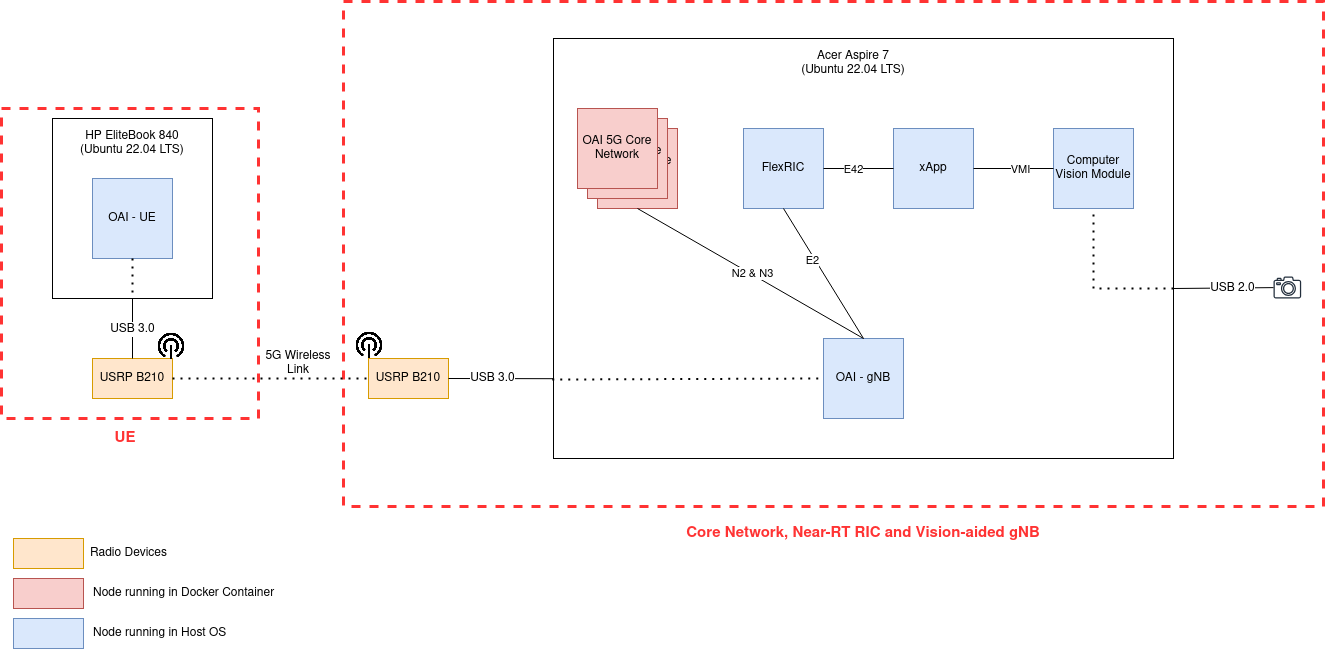
\includegraphics[width=0.7\linewidth]{figures/System Arch.drawio}
    \caption[System architecture designed for implementing and evaluating the proposed solution]{System architecture designed for implementing and evaluating the proposed solution.}
    \label{fig:design_arch}
\end{figure}

The following subsections detail the hardware used in the implementation and the choices for software packages.


\subsection{Software}\label{subsec:software}
This section presents the main software packages used to develop the Vision Module and implement the 5G network.
Beyond this, in the repository containing the VM, there is a file for reproducing the Python virtual environment.

\subsubsection{OpenCV}
% revision
There are several open-source software packages available for Computer Vision in Python.
Open Source Computer Vision Library (OpenCV)~\cite{opencv} is one of them.
It contains several optimized algorithms, which can be used for different tasks, including object detection, image processing, and real-time video analysis.
This diverse support makes it suitable for both basic tasks and complex applications requiring advanced functionalities.
Moreover, OpenCV's well-documented API facilitates ease of use and integration into various projects, ensuring efficient development and deployment.
Unlike some other libraries that may focus on specific aspects of image processing or lack support across different domains, OpenCV provides a solution with cross-platform compatibility, making it applicable across diverse operating systems and hardware setups.
Furthermore, OpenCV benefits from a large and active community, offering extensive resources, tutorials, and community support, which are invaluable for developers and researchers seeking assistance or collaboration in tackling complex computer vision challenges effectively and efficiently.
Therefore, OpenCV is the leading choice for robust and scalable computer vision applications.

Additionally, OpenCV is the only library who directly supports ArUco Markers.
ArUco is a widely-used open-source library for Augmented Reality (AR) applications that involves detecting and tracking augmented markers.
These markers are specially designed square or rectangular patterns with a unique binary encoding, which can be printed and placed in the physical environment.
ArUco markers are typically used in computer vision tasks to provide reference points in a scene, enabling accurate localization and tracking of objects or video cameras.

OpenCV emerges as the premier choice among general computer vision libraries, distinguished by its extensive feature set, optimized performance, and robust community support.
Unlike scikit-image~\cite{Scikit-learn}, which excels in image processing tasks with functions for filtering, morphology, and segmentation, OpenCV offers a broader range of over 2500 optimized algorithms spanning image and video processing, object detection, and video camera calibration.
In contrast to Pillow (PIL Fork)~\cite{pillow}, which specializes in image format handling and basic manipulation, OpenCV provides comprehensive tools for both foundational and advanced computer vision applications.
Moreover, while SimpleCV~\cite{simplecv} simplifies OpenCV usage with a user-friendly interface, OpenCV's C++ backend and GPU acceleration capabilities enable superior performance, which is crucial for real-time processing and large-scale data operations.

In our proposed solution, OpenCV is utilized to:
\begin{itemize}
    \item \textbf{Obtain Frames:} OpenCV is used to capture video frames from the video camera.
    It provides easy-to-use interfaces to capture and manipulate video streams from various input sources.
    \item \textbf{Detect ArUco Markers:} OpenCV includes modules for detecting ArUco markers, which are widely used in computer vision applications for video camera calibration, pose estimation, and augmented reality.
    In our solution, these markers help in identifying the UEs without the need to train the YOLO model to perceive such objects.
\end{itemize}

\subsubsection{Ultralytics YOLO}
As discussed in Section ~\ref{sec:CV}, Ultralytics YOLO (You Only Look Once)~\cite{ultralytics_docs} is a state-of-the-art, real-time object detection solution.
It is known for its speed and accuracy, making it suitable for applications that require fast and reliable object detection and tracking.
While there are other solutions, also presented in that Section, we chose Ultralytics YOLO due to simplicity, integration and since it is suitable for the intended application and use in state-of-the-art object detection and tracking situations.

In our proposed solution, Ultralytics YOLO is employed to:
\begin{itemize}
    \item \textbf{Detection:} YOLO is used to detect various objects in the frames captured by the video camera.
    Its real-time capabilities allow for the immediate identification of obstacles within the field of view.
    \item \textbf{Tracking:} YOLO’s tracking module is used to keep track of detected objects over successive frames.
    This is crucial for maintaining the continuity of object identification and for predicting future positions of the obstacles. %BOTSORT and BYTETRACK
\end{itemize}

The combination of OpenCV and Ultralytics YOLO allows for robust detection, tracking, and message exchange functionalities in our vision module.
OpenCV handles the initial capture and processing of video frames, while YOLO and BoT-SORT performs the real-time detection and tracking of objects.
This integrated approach ensures that the vision module can effectively monitor and report on obstacles, providing key information to subscribed services.

\subsubsection{ASN1Tools and ASN1C}
There are a few open-source libraries available for handling ASN.1.
FlexRIC utilizes asn1c~\cite{asn1c}, so for simplicity we chose the same for the xApp (client).
asn1c is a open-source ASN.1 compiler that generated C/C++ code for ASN.1 data structures, supporting different encoding rules.
While this library also supports Python, we chose not to use it, since there are simpler APIs specially tailored for Python development.
As for the Vision Module (Python server), we chose ASN1Tools because it offers certain advantages.

ASN1Tools~\cite{asn1tools} is a Python library provides a simple way to handle ASN.1 data structures, through a straightforward API\@.
The library support for a range of ASN.1 specifications and encoding rules, including BER, DER, and PER\@.
Moreover, ASN1Tools is actively maintained, with regular updates and improvements.
This guarantees that we have access to the latest features and bug fixes, which enhances the reliability and stability of our system.
ASN1Tools is optimized for performance, allowing for fast encoding and decoding operations.
This optimization is suited for real-time applications like our Vision Module, where processing speed is essential to maintain system responsiveness and accuracy.

While other libraries such as pyasn1~\cite{pyasn1} and libtasn1~\cite{libtasn1} are available, they have certain limitations.
pyasn1, for instance, is less efficient in terms of performance and has a more complex API\@.
libtasn1, part of the GNU project, is less user-friendly and optimized for performance.


\subsubsection{5G Core Network, 5G gNB, and 5G UE}
The main open-source 5G software packages for implementing an O-RAN based architecture are OAI~\cite{openairinterface} and srsRAN~\cite{srslte}.
For our system, we chose OAI because it provides all the necessary components to deploy a 5G standalone network, including both the RAN and Core network.
In contrast, srsRAN only supports the deployment of the RAN, requiring an additional software package, such as OAI, to implement the Core network.

\subsubsection{Near-RT RIC}
The main open-source software packages able to implement a Near-RT RIC are Mosaic5G’s FlexRIC~\cite{flexric} and  O-RAN Software Community’s Near-RT RIC~\cite{oran-sc}.
FlexRIC was chosen for our solution due to its lightweight nature, launched from an executable file.

In contrast, the O-RAN RIC presents a disadvantage in terms of its complexity and resource requirements.
It often demands more substantial computational resources and a more involved setup process, which is a significant drawback for our solution.

\subsection{Hardware}\label{subsec:hardware}


\subsubsection{Core Network, FlexRIC, Computer Vision module and gNB}
The OAI Core Network, FlexRIC,the Computer Vision module and the gNB were deployed in a laptop Acer Aspire A715-74G, show in Figure~\ref{fig:computer_acer}.
The OAI Core was deployed using Docker containers, requiring 4 cores CPU, 16GB of RAM and a minimum of 1.5GB free storage for the docker images.
As for FlexRIC, it does not have hardware requirements listed, but while deploying it was noticed that it is not resource intensive, sufficing the same ones required for the Core Network.
The xApp was deployed alongside FlexRIC in order to assure reduced latency between the two components.
Also,  the way interface E42 is implemented requires them to be running in the same computing unit.
As for the gNB, the hardware recommended are 8 physical CPU cores and 32 GB of RAM\@.
While the laptop used did not fulfill these requirements, it has proven sufficient to run the OAI gNB software, as it was noted before in~\cite{queiros2023autonomous}.

\begin{figure}[H]
    \centering
    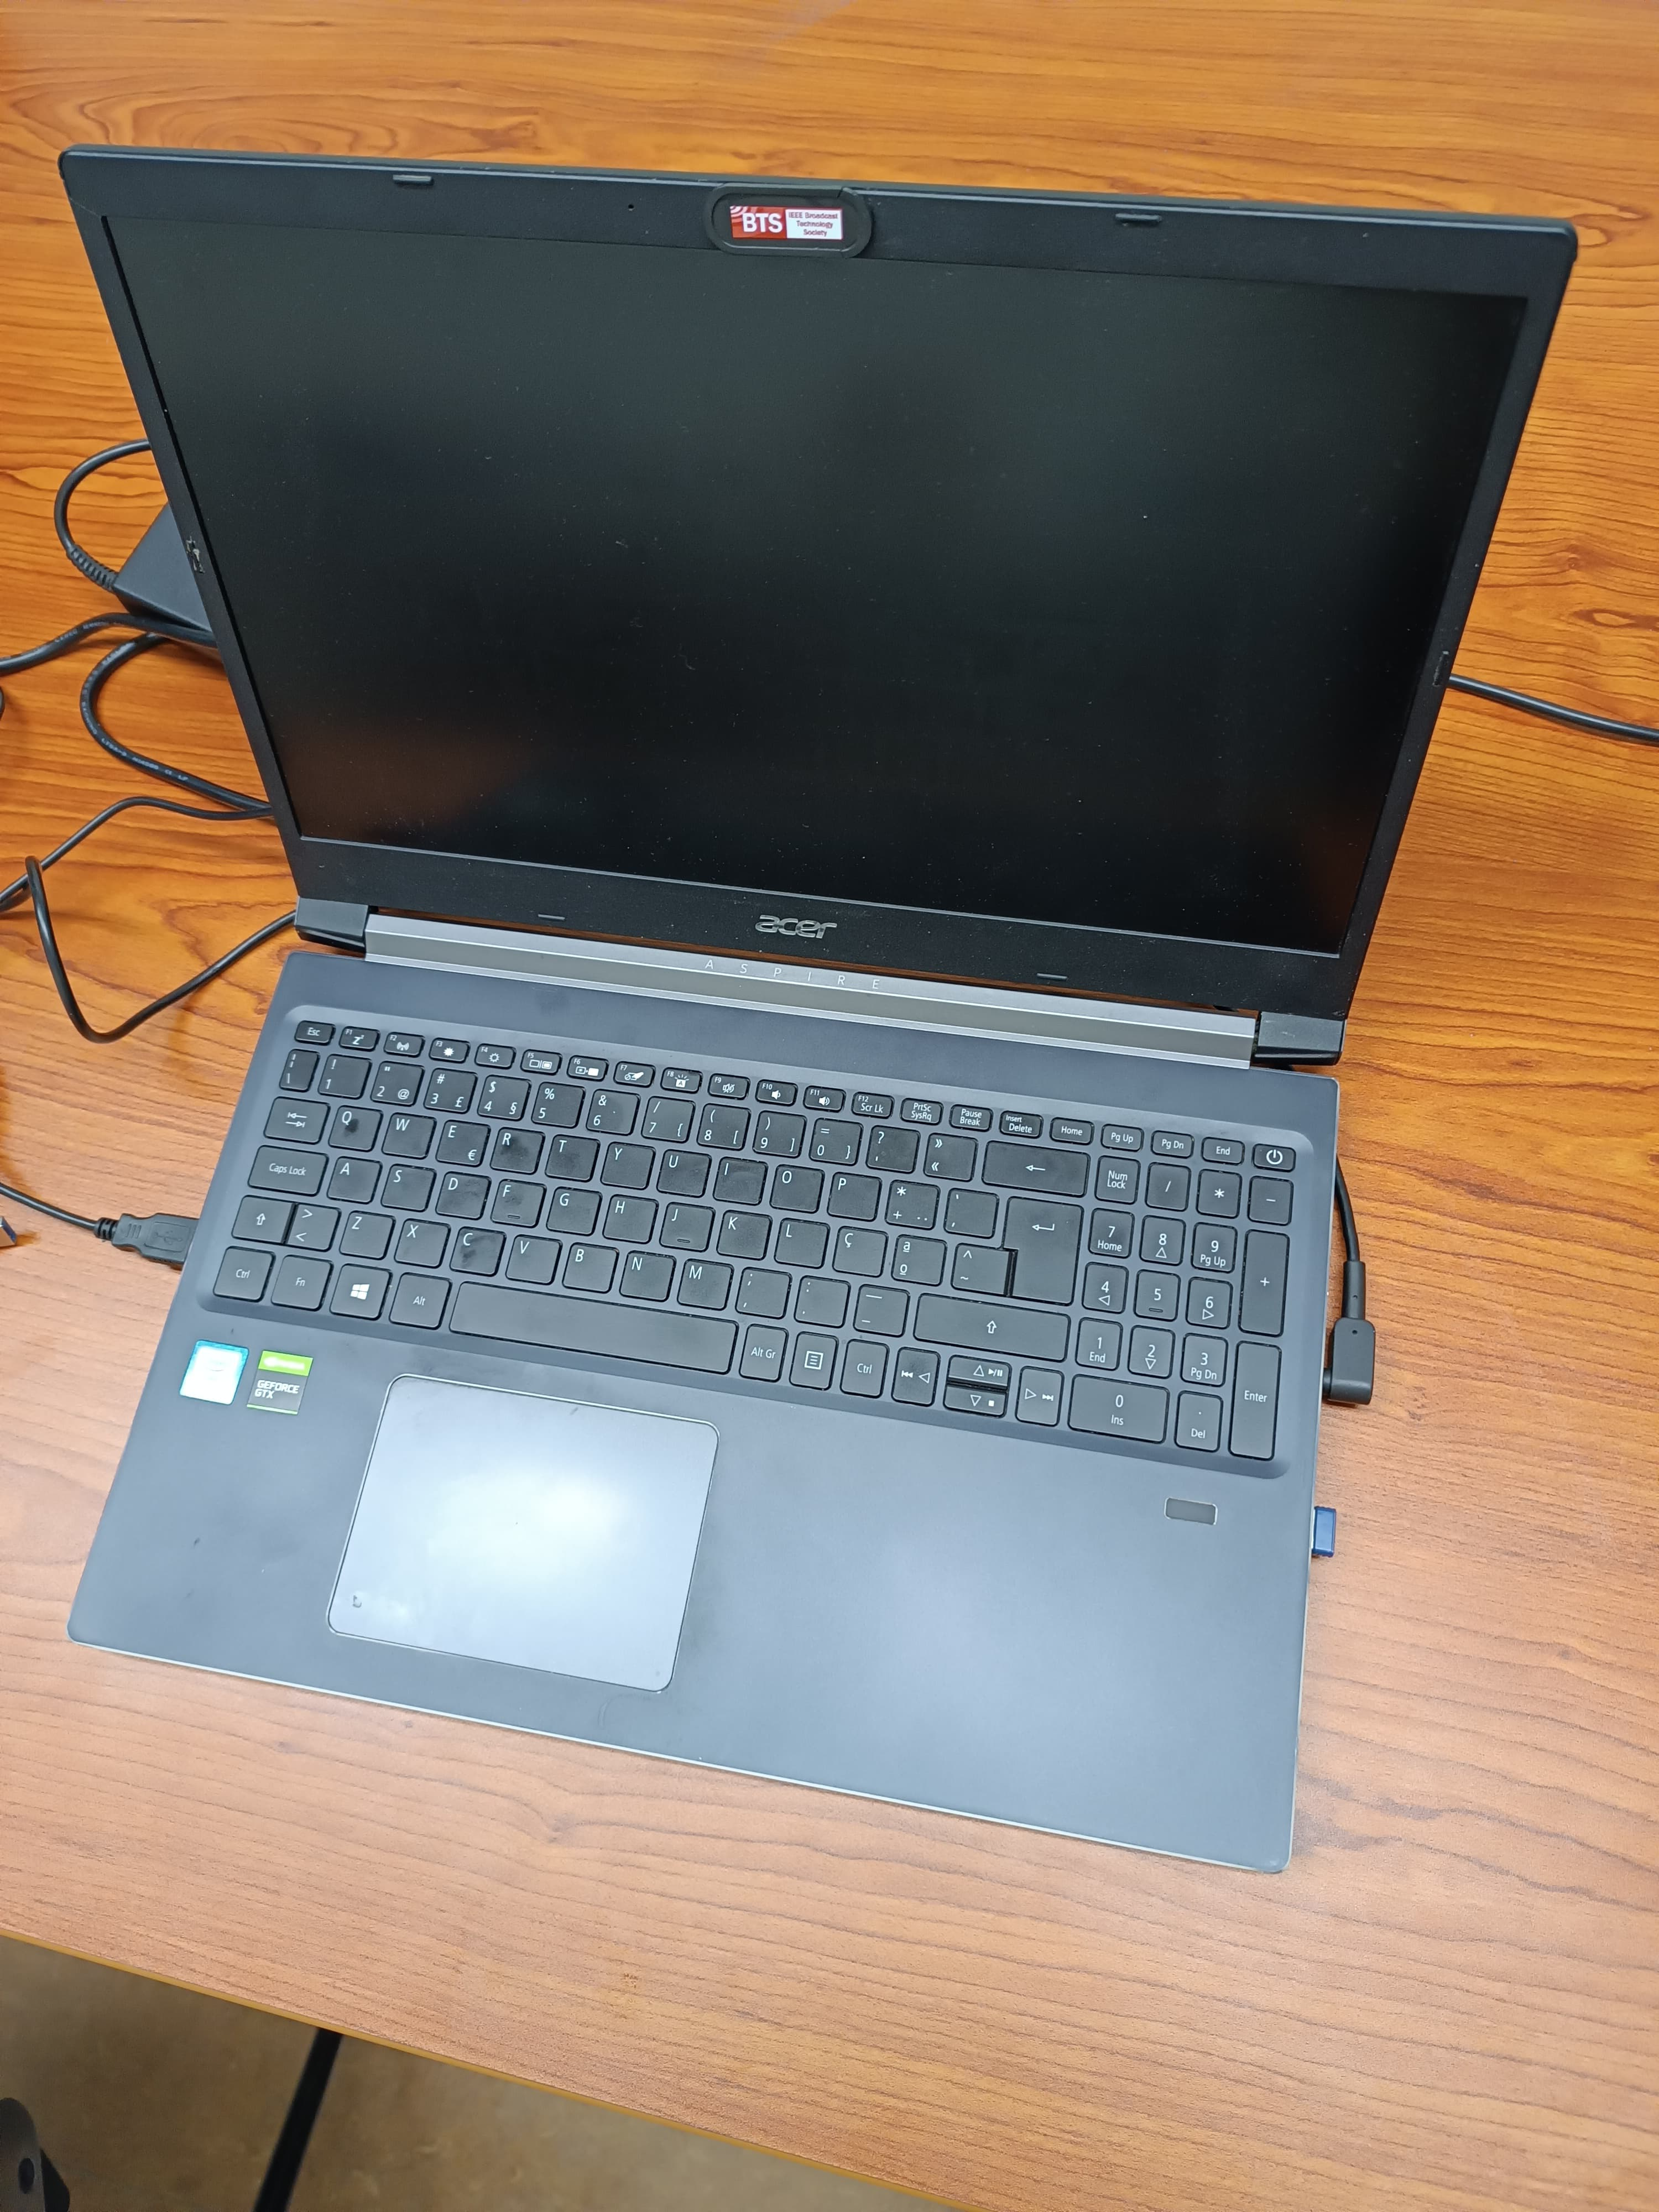
\includegraphics[width=0.3\linewidth]{figures/acer}
    \caption{Acer Aspire A715-74G Laptop}
    \label{fig:computer_acer}
\end{figure}

As for the Computer Vision Module, the minimal hardware requirement is a CUDA-compatible GPU ~\cite{ultralytics_faq}, for Ultralytics YOLO model to properly run.
Given that for our solution a pre-trained model has proven enough to accurately detect and track objects, we did not necessitate great GPU capacity to train a model.

Table ~\ref{tab:specs_pc} presents the specification of the computer.

\begin{table}[H]
    \caption{Specifications of the Acer Aspire A715-74G.}
    \label{tab:specs_pc}
    \begin{tabular}{|c|c|}
        \hline
        \textbf{Specification} & \textbf{Details} \\ \hline
        Processor                      &           Intel(R) Core(TM) i5-9300H CPU @ 2.40GHz   \\ \hline
        RAM                      &          16GB        \\ \hline
        Disk                      &   2 SSDs  512GB and 256GB         \\ \hline
        GPU                     &   GeForce GTX 1050 (3GB)      \\ \hline
        Operational System & Ubuntu 22.04.4 LTS                  \\ \hline
    \end{tabular}
\end{table}

For the Computer Vision Module, we opted to use a webcam due to its simplicity and ease of integration.
The chosen was a model LL-4196, offering Full HD (1920 x 1080 Pixels) resolution and supporting a frame rate of 30 FPS\@.
This ensures that the video feed acquired is of high quality, providing sufficient detail and smooth motion necessary for accurate computer vision processing.
The camera connects to the computer using a USB 2.0 interface.
Figure \ref{fig:camera} shows the video camera and its USB interface.

\begin{figure}[H]
    \centering
    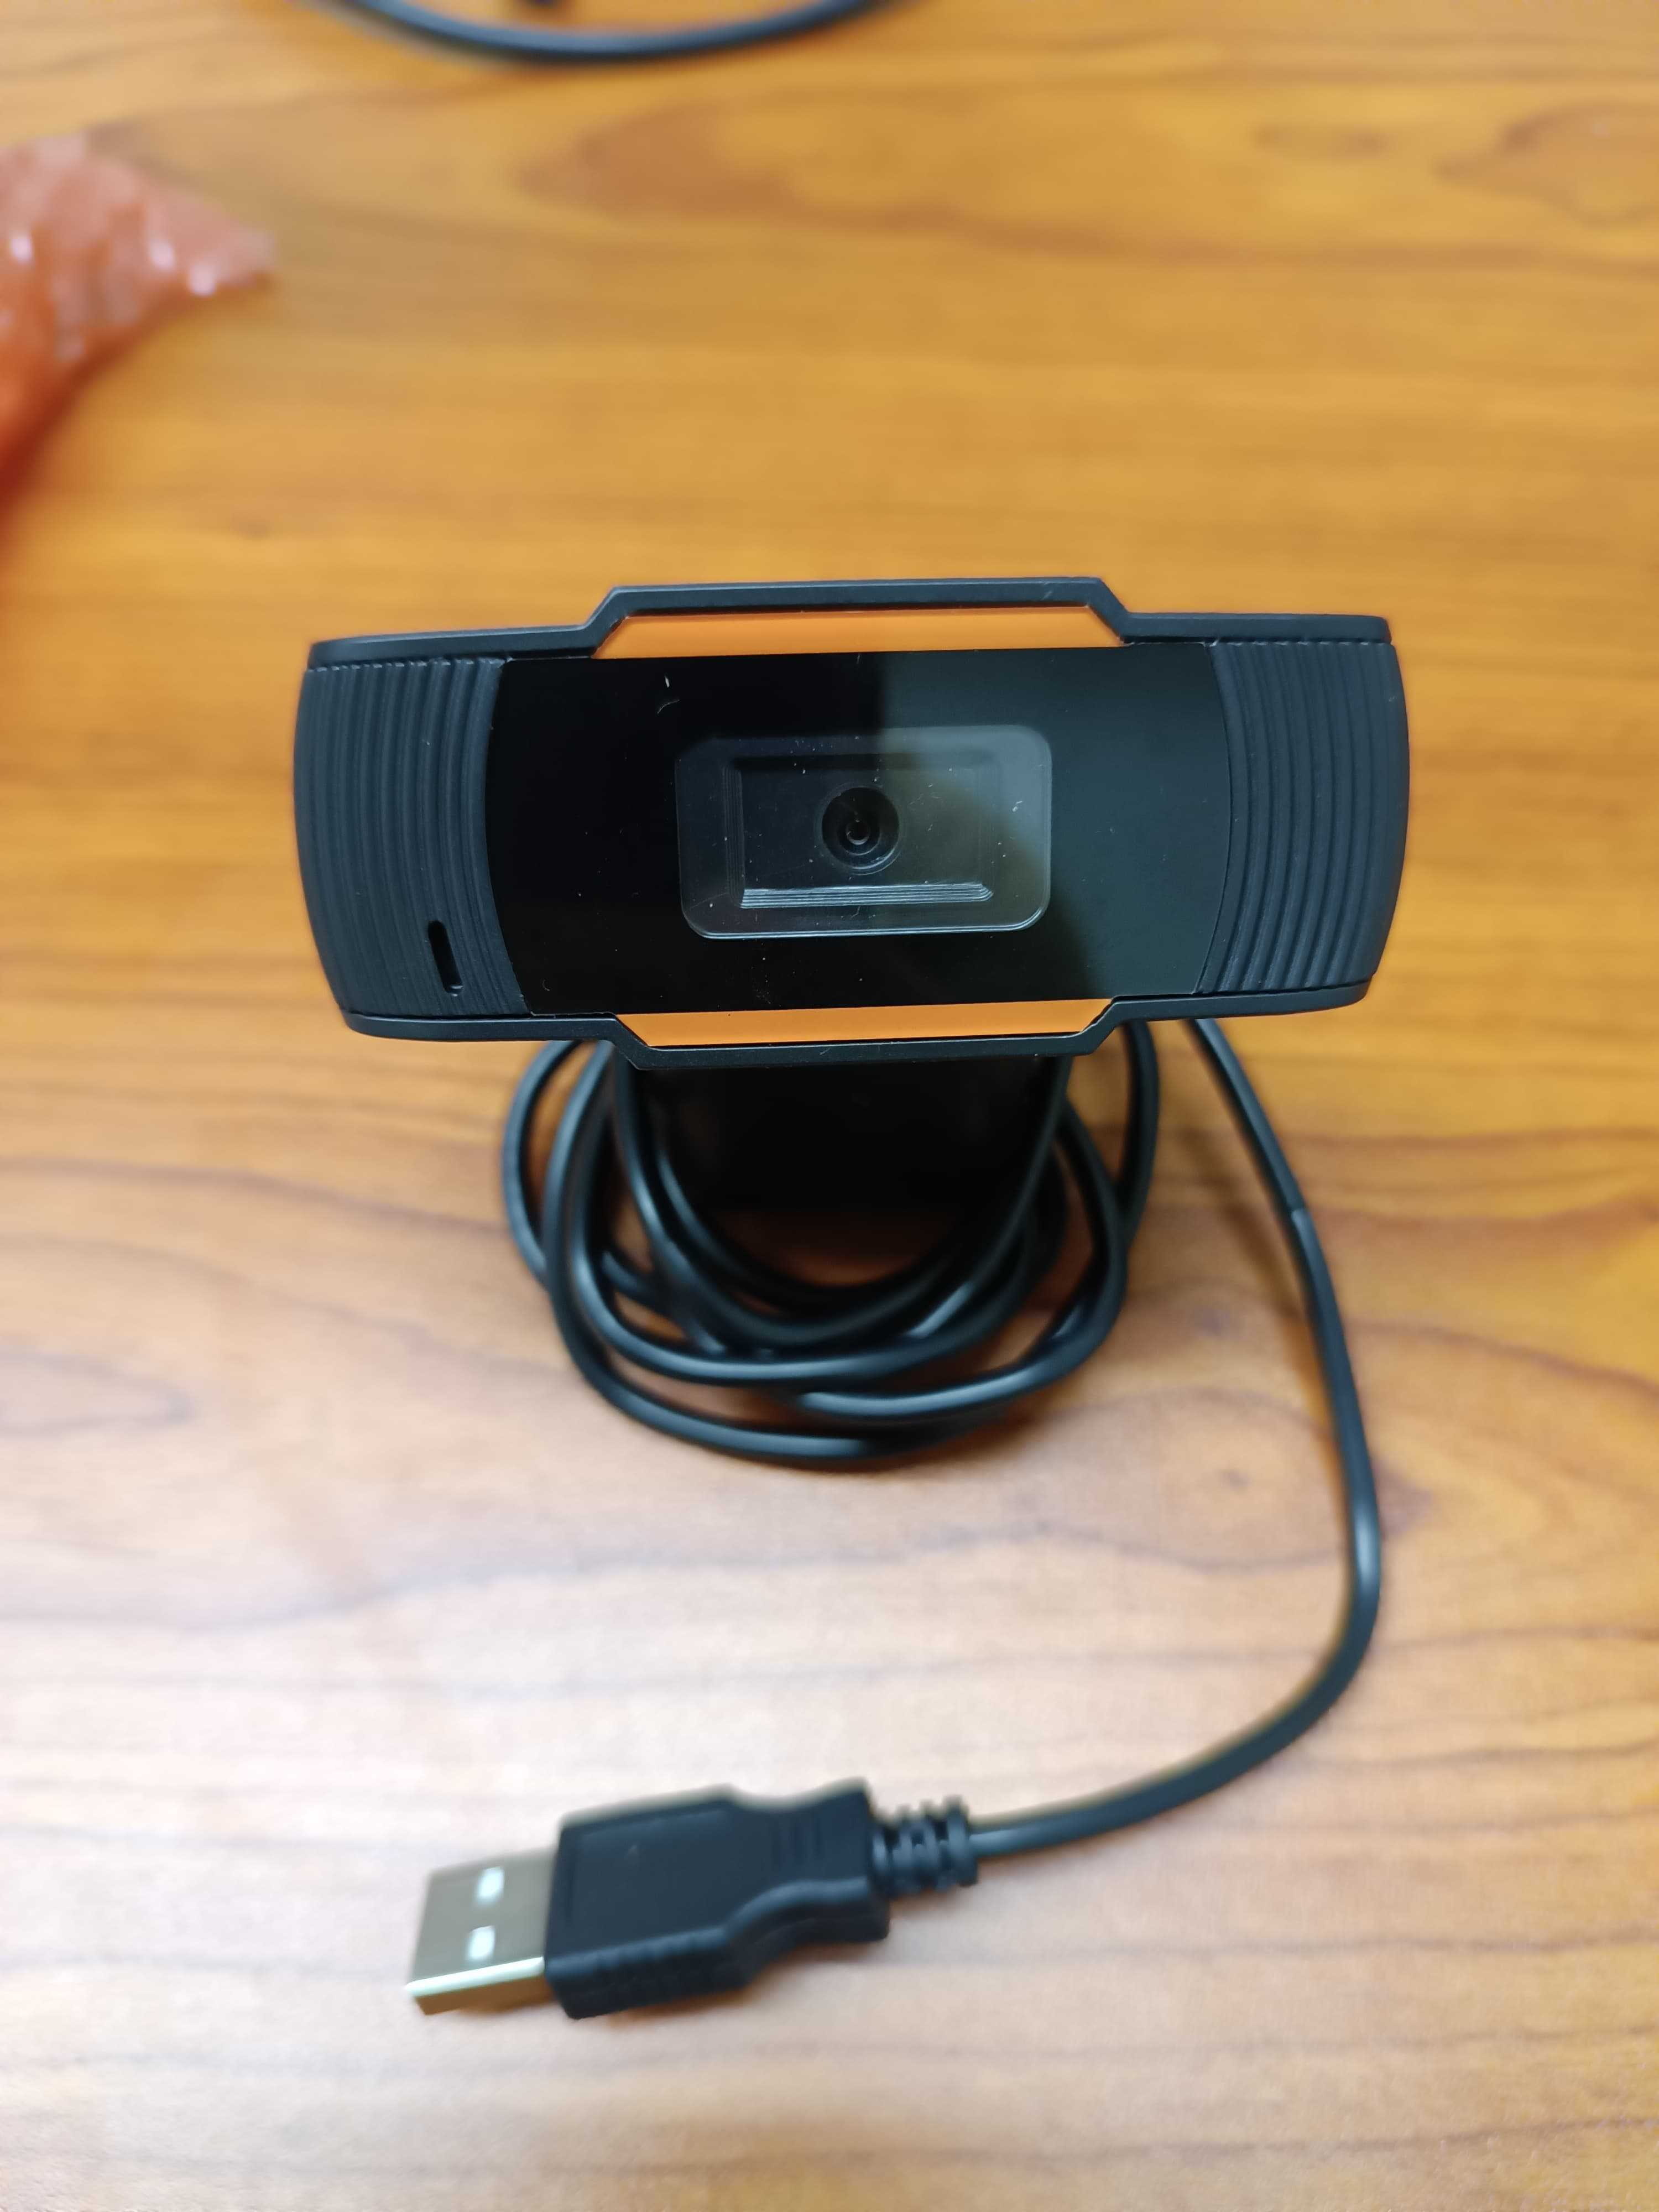
\includegraphics[width=0.3\linewidth]{figures/webcam}
    \caption{Webcam used to capture the video.}
    \label{fig:camera}
\end{figure}

Deploying the gNB and the UE in two different host computers implicates the use of Software-Defined Radio (SDR) in order to establish a 5G connection between the gNB and the UE\@.
OAI recommends the use of three SDR models: USRP B210, USRP N300 and USRP X300\@ \cite{openairinterface_tutorial}.
For our implementation, we have selected the first since it is cost-effective and a popularity across the community.
This model uses a USB 3.0 interface to connect to the computer acting as a processing unit.
The SDR was equipped with two W5208K dipole antennas.
Figure~\ref{fig:SDRs} shows the two SDRs with their respective antennas.
We have selected 3.6GHz as the carrier frequency for the 5G RAN\@.

\begin{figure}[H]
    \centering
    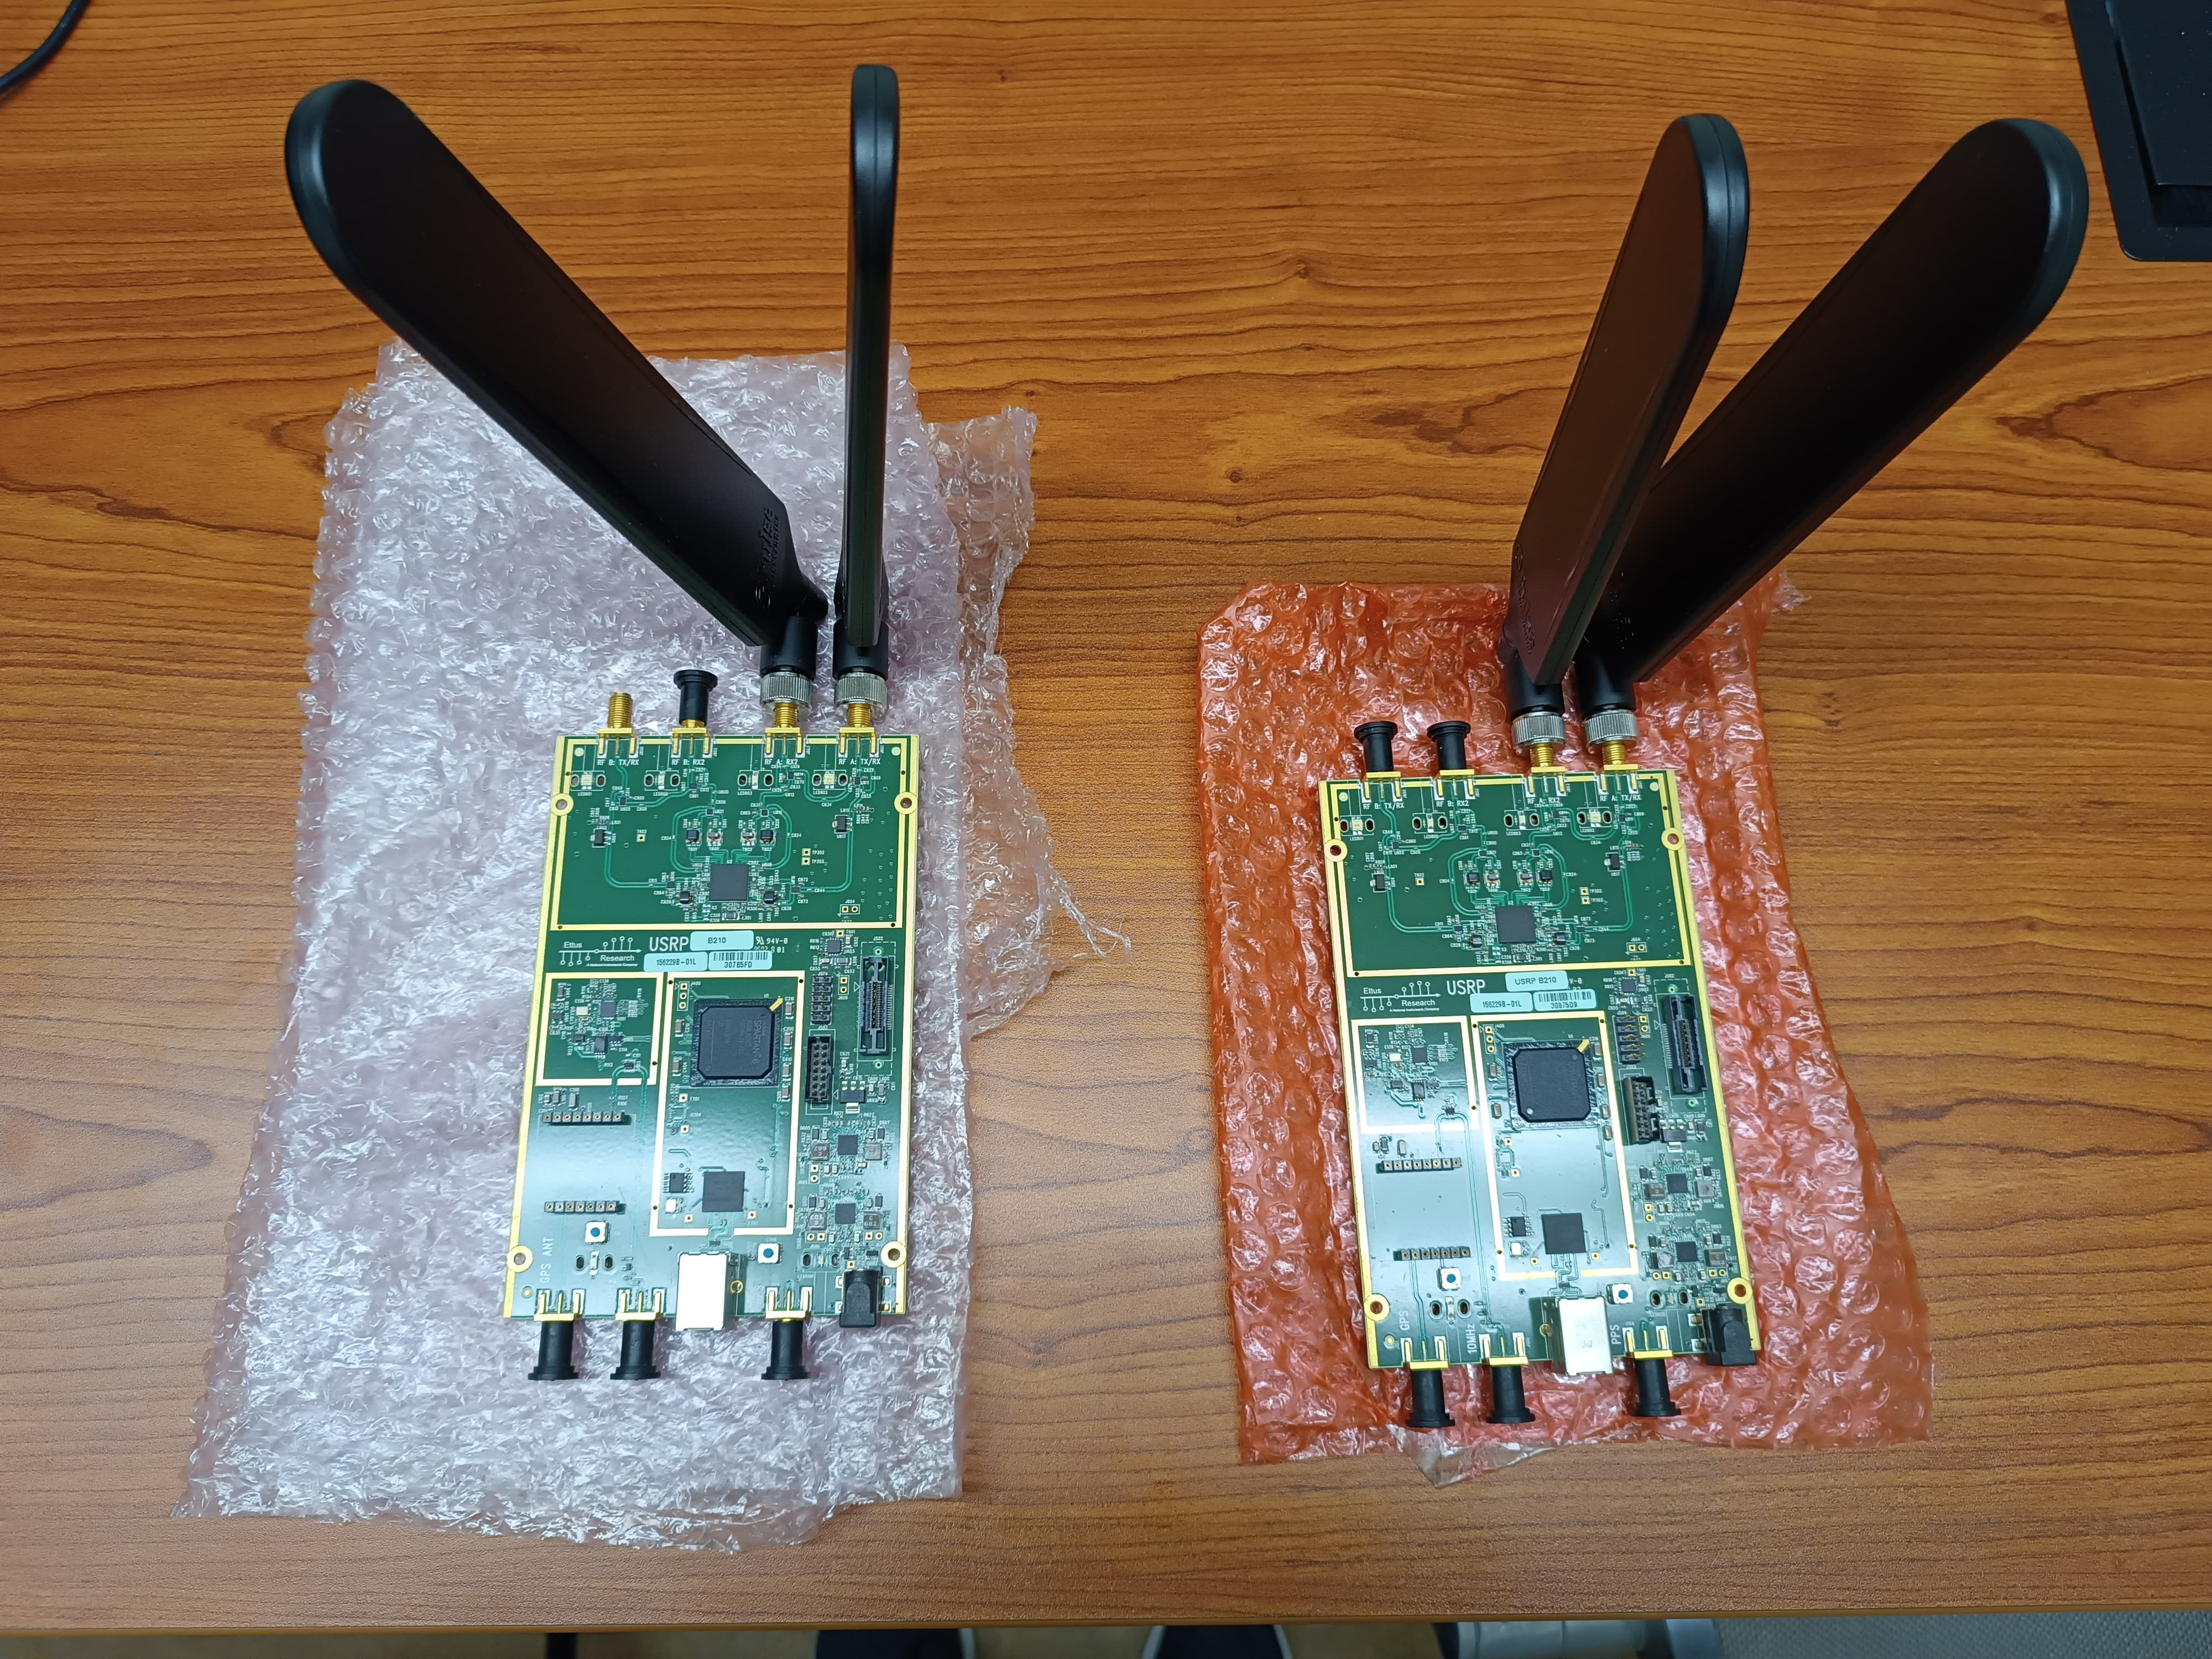
\includegraphics[width=0.5\linewidth]{figures/SDRs}
    \caption{USRP B210 SDRs and their respective antennas.}
    \label{fig:SDRs}
\end{figure}



\subsubsection{UE}
The UE was deployed in HP EliteBook 840 Laptop, shown in Figure~\ref{fig:computer_hp}.
The hardware requirements for the deployment of the UE are 8 cores and 8GB of RAM\@.
Table~\ref{tab:specs_pc_ue} depicts the specification of the computer responsible for the UE\@, showcasing that the hardware is enough to run the UE application.

\begin{figure}[H]
    \centering
    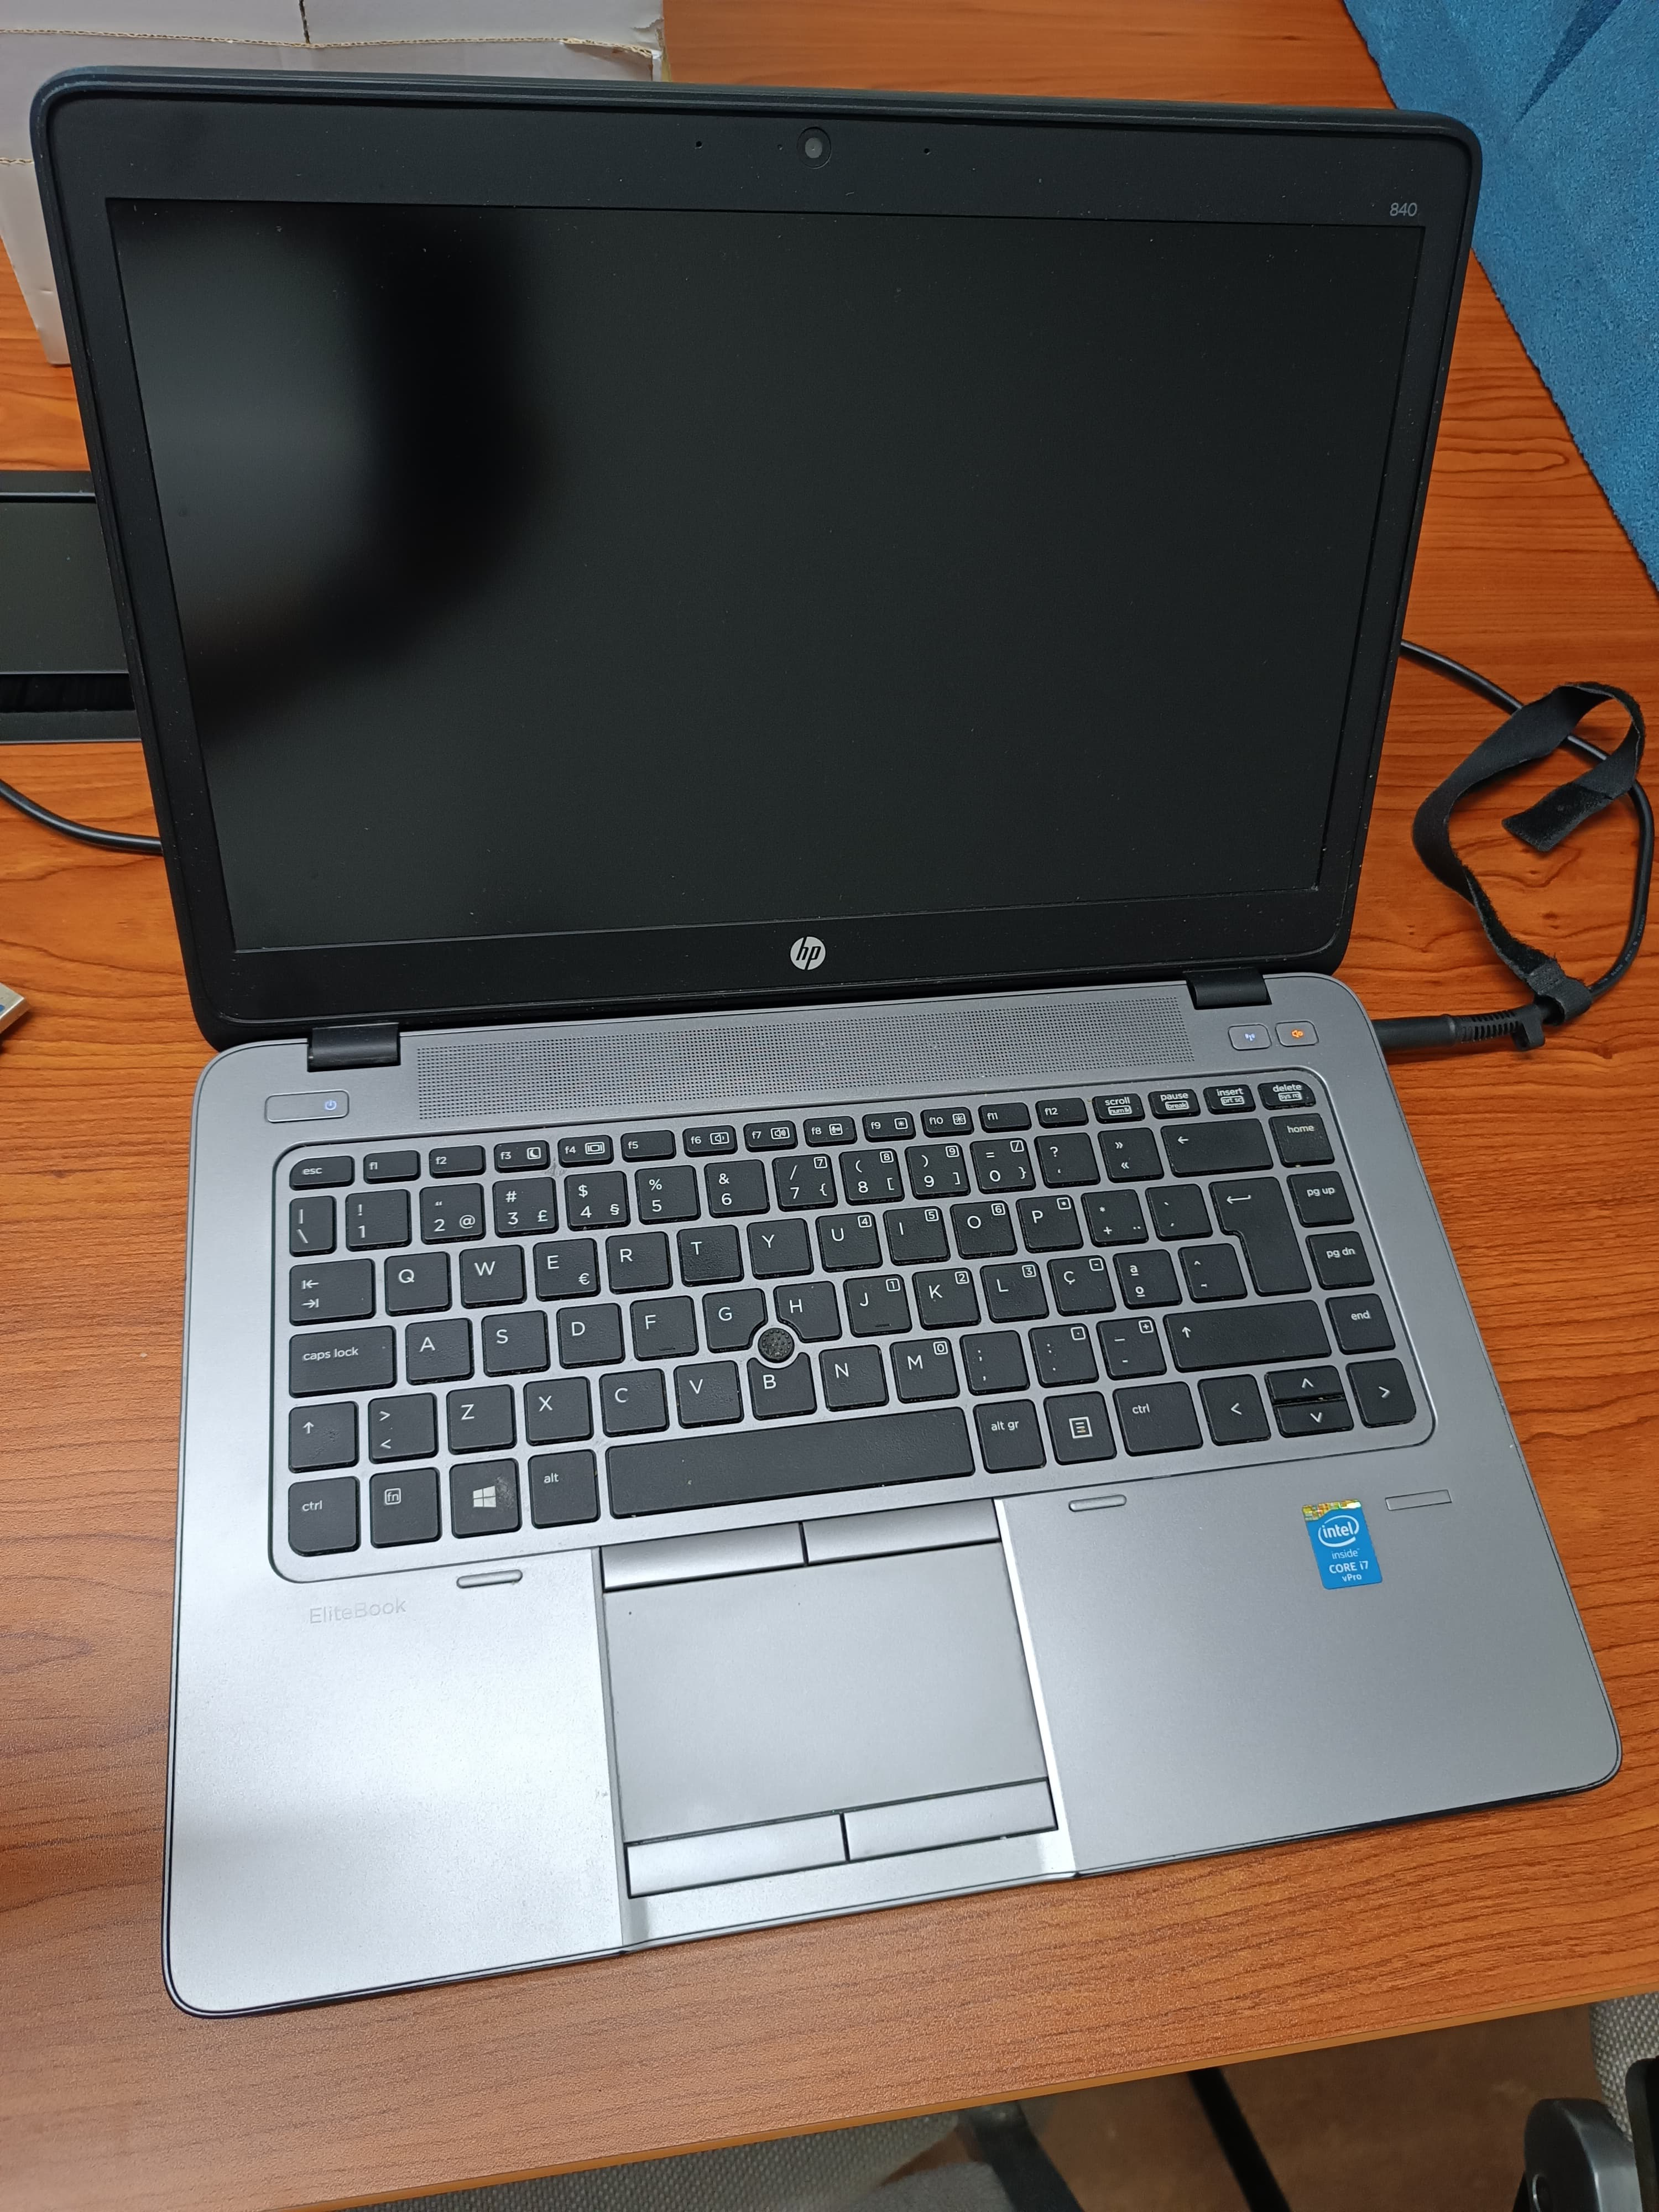
\includegraphics[width=0.3\linewidth]{figures/hp}
    \caption{HP EliteBook 840 Laptop}
    \label{fig:computer_hp}
\end{figure}

\begin{table}[H]
    \caption{Specifications of the HP EliteBook 840.}
    \label{tab:specs_pc_ue}
    \begin{tabular}{|c|c|}
        \hline
        \textbf{Specification} & \textbf{Details} \\ \hline
        Processor                      &  Intel(R) Core(TM) i7-5600U CPU @ 2.60GHz          \\ \hline
        RAM                      &          16GB        \\ \hline
        Disk                      &   128GB         \\ \hline
        GPU                     &   Intel Corporation HD Graphics 5500                \\ \hline
        Operational System & Ubuntu 22.04.4 LTS                  \\ \hline  %  check
    \end{tabular}
\end{table}

\section{System Implementation}\label{sec:impl}

\subsection{Vision Module}\label{subsec:vision-module}
Our vision module is implemented as a Python server, designed to interface with the xApp (its client) via an SCTP socket over the Loopback interface (127.0.0.1) on port 4321.
The module is designed to manage multiple functions efficiently, including:

\begin{itemize}
\item Information Exchange: Facilitates communication between the server and client.
\item Detection and Tracking: Identifies and tracks objects within the video feed.
\item Image Processing: Processes video data to derive meaningful insights.
\item Utility Operations: Performs various supportive tasks to enhance overall functionality.
\end{itemize}

To ensure timely and efficient video processing, we utilize a multi-threading approach:

\begin{enumerate}
\item Communication Thread: Manages the connection with the client, handling message exchanges and maintaining seamless communication.
\item Processing Thread: Focuses on video analysis, including object identification and generating messages based on the environmental data processed from the video stream.
\end{enumerate}

For optimized performance in handling the computationally intensive tasks of image processing, we leverage GPU acceleration.
Specifically, we use the Ultralytics YOLOv8n model.
We selected the nano version, YOLOv8n, due to its reduced parameter count, which makes it less resource-intensive and better suited to our use case.
This choice significantly accelerates processing times and reduces CPU load, leading to enhanced overall system efficiency and responsiveness.
The combination of GPU utilization and the streamlined YOLOv8n model ensures that our module operates effectively even under high-demand conditions.



\subsection{OAI 5G Core Network}\label{subsec:oai-5g-core-network}
OAI offers three methods for implementing the Core Network: bare-metal installation or virtual machines, automated deployment of network functions (NFs) in Docker containers using Docker-Compose, and cloud-native deployment using Helm Chart on OpenShift or Kubernetes clusters ~\cite{oai5gcore}.
Choosing Docker for deployment simplifies the process by encapsulating network functions in containers, making them easier to manage, scale, and automate, which enhances the overall efficiency and flexibility of the network infrastructure.
Figure~\ref{fig:core_depl} shows the deployed 5G Core diagram.
The IP addresses for each Core Network component and Data Network and can be seen respectively in Tables~\ref{tab:ip_core} and~\ref{tab:ip_dn}.


\begin{figure}[H]
    \centering
    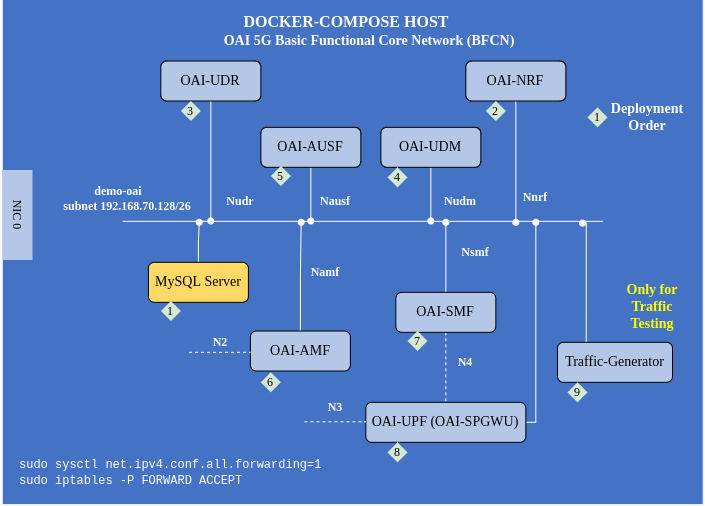
\includegraphics[width=0.7\linewidth]{figures/core_deply}
    \caption{Core deployment diagram~\cite{oai_cn5g_fed_deploy}.}
    \label{fig:core_depl}
\end{figure}


\begin{table}[H]
    \caption{Deployed 5G Core Network Functions IP addresses.}
    \label{tab:ip_core}
    \centering
    \resizebox{0.3\textwidth}{!}{%
        \begin{tabular}{|c|c|}
            \hline
            \textbf{Core Network Function} & \textbf{IP} \\ \hline
            NRF & 192.168.70.130 \\ \hline
            MySQL & 192.168.70.131\\ \hline
            AMF & 192.168.70.132 \\ \hline
            SMF & 192.168.70.133 \\ \hline
            UPF & 192.168.70.134 \\ \hline
            UDR & 192.168.70.136 \\ \hline
            UDM & 192.168.70.137 \\ \hline
            AUSF & 192.168.70.138 \\ \hline
        \end{tabular}}
\end{table}

\begin{table}[H]
    \caption{Deployed Data Network Components IP addresses.}
    \label{tab:ip_dn}
    \centering
    \resizebox{0.3\textwidth}{!}{%
        \begin{tabular}{|c|c|}
            \hline
            \textbf{Core Network Function} & \textbf{IP} \\ \hline
            UPF & 192.168.70.134 \\ \hline
            External-DN & 192.168.70.135 \\ \hline
        \end{tabular}}
\end{table}






\subsection{OAI gNB}\label{subsec:oai-gnb}
The deployment of the OAI gNB, we used the latest version of OAI RAN, following the steps present in~\ref{openairinterface5g_e2ap}.
Other than the steps described in the tutorial, in order to deploy the gNB with the SDR, it was required to do some alterations to \textit{gnb.sa.band78
.fr1.106PRB.usrpb210.conf} configuration file.
Namely, edit MCC, MNC and TAC values to assure they corresponded to the values present in the Core \textit{docker-compose.yaml} file.
Figure~\ref{fig:gnb_conf} depicts the alterations, in lines 13 and 14 of the file to comply with the Core values.
If these values do not align, the NGAP setup between AMF and gNB over N2 interface will fail.
It is also necessary to modify the IP address of the AMF and an IP so that the gNB can communicate with the AMF and SMF\@.

\begin{figure}[H]
    \centering
    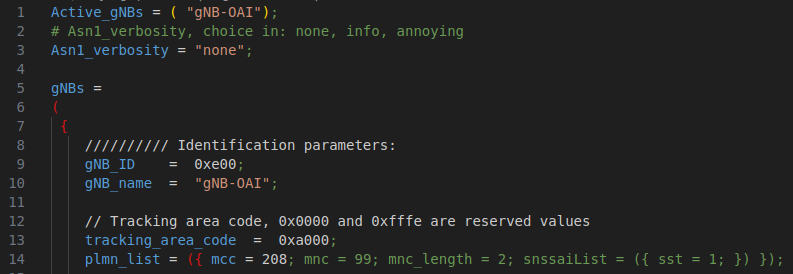
\includegraphics[width=0.7\linewidth]{figures/gnb_conf}
    \caption{.}
    \label{fig:gnb_conf}
\end{figure}

\textcolor{red}{CONTINUE}

Finally, it is necessary to establish a connection between the OAI gNB software and the SDR\@.
As recommended by OAI, we utilized the USRP Hardware Driver (UHD)~\cite{uhdusrpdriver}.
UHD is a driver that enables communication between software and USRP hardware, providing a standardized interface for configuring and controlling aspects of the SDR devices, such as frequency, sample rate, gain, and antenna settings.
Figure~\ref{fig:uhd_probe} illustrates the UHD driver detecting the USRP device, loading its firmware, and performing diagnostic tests.

\begin{figure}[H]
    \centering
    
\includegraphics[width=0.7\linewidth]{figures/uporto-feup}
    \caption{UHD obtaining information about the connected USRP device and testing it}
    \label{fig:uhd_probe}
\end{figure}

\subsection{OAI 5G UE}\label{subsec:oai-5g-ue}
In order to deploy the OAI UE, we needed to initiate the OAI UE software modem with parameters corresponding to the gNB settings.
The command used is as follows:

\lstinline[columns=flexible,breaklines=true]{sudo ./nr-uesoftmodem -r 106 --numerology 1 --band 78 -C 3619200000 --ue-fo-compensation --sa -E --uicc0.imsi 208990200000001}


The parameters are:

\begin{itemize}
    \item \texttt{-r 106}: Sets the radio configuration to 106.
    This must match the radio configuration set on the gNB to ensure proper communication.
    \item \texttt{--numerology 1}: Specifies the numerology index, set to 1, defining sub carrier spacing and slot duration.
    The gNB must use the same numerology index for compatibility.
    \item \texttt{--band 78}: Configures the UE to operate in the n78 band.
    The gNB is also set to operate in the n78 band, facilitating the connection.
    \item \texttt{-C 3619200000}: Sets the center frequency to 3619.2 MHz. The gNB is configured to transmit on this same center frequency.
    \item \texttt{--ue-fo-compensation}: Enables frequency offset compensation for the UE, ensuring synchronization with the gNB.
    \item \texttt{--sa}: Indicates that the UE is operating in standalone mode, directly connecting to the 5G network without relying on an LTE anchor, matching the gNB configuration.
    \item \texttt{-E}: Specifies that the program should utilize 75\% of the sampling rate frequency.
    \item \texttt{--uicc0.imsi 208990200000001}: Sets the IMSI for the UE to \texttt{208990200000001}.
\end{itemize}

We needed to use one of the International Mobile Subscriber Identity (IMSI) values present in the Core database to ensure that the UE could authenticate successfully.
The IMSI value, \texttt{208990200000001}, was selected from the Core database and used in the \texttt{nr-uesoftmodem} command.
This selection was crucial because it aligns with the subscriber information stored in the network, facilitating proper authentication and allowing the UE to connect and communicate with the network.
By ensuring that the IMSI used in the UE configuration matches an entry in the Core database, we verify that the UE can be authenticated correctly and allowed access to the network services.

If we use an IMSI value that is not present in the Core database, the authentication process will fail, as illustrated by the Wireshark capture shown in Figure~\ref{fig:UE_failure}.

\begin{figure}[H]
    \centering
    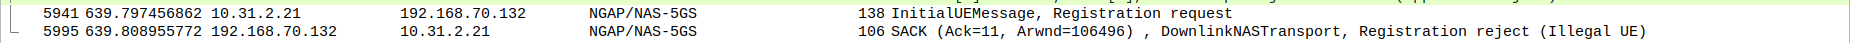
\includegraphics[width=\linewidth]{figures/Ue_fail}
    \caption{UE registration rejected due to UE SIM details}
    \label{fig:UE_failure}
\end{figure}

\subsection{FlexRIC}\label{subsec:flexric}
FlexRIC is deployed in the same computer as the OAI 5G Core Network.
The procedure is to install the required dependencies and compile FlexRIC software.
By default, FlexRIC is configured to run on the Loopback Interface address (127.0.0.1).
Since we are deploying gNB and FlexRIC in the same Host, this is not necessary to change.
In order to assure the use of the E2 Agent, is necessary to include in the configuration file of the gNB the following:

\begin{verbatim}
e2_agent = {
  near_ric_ip_addr = "127.0.0.1";
  sm_dir = "/usr/local/lib/flexric/"
}
\end{verbatim}

This informs that FlexRIC is running on the localhost IP, indicating that the RIC is running on the same machine as the E2 agent.
The directory informs where the Service Models for FlexRIC are located.
This is essential to assure the correct communication between OAI gNB and FlexRIC\@.



\section{Summary}\label{sec:summary}
Our proposed architecture is divided into two logical units.
The first one comprises the OAI 5G Core Network, FlexRIC, xApp and Vision Module, deployed in an Acer Aspire Laptop.
The second unit comprehends the OAI UE, deployed in an HP Elitebook.
The gNB and the UE used USRP B210 SDR board to connect via 5G Wireless Link.
The Vision Module received a video feed, processed it and sent relevant obstacle information seen in the video, via its interface.
The xApp was responsible for monitoring the received messages and the SNR.
The chapter demonstrates the feasibility and benefits of integrating computer vision with mobile communications.
By leveraging Computer Vision, the quality of the communication channel can be enhanced.






